\documentclass[onlymath]{beamer}
% \documentclass[onlymath,handout]{beamer}

% Macros used by all lectures, but not necessarily by excercises

%%% General setup and dependencies:

% \usetheme[ddcfooter,nosectionnum]{tud}
\usetheme[nosectionnum,pagenum,noheader]{tud}
% \usetheme[nosectionnum,pagenum]{tud}

% Increase body font size to a sane level:
\let\origframetitle\frametitle
% \renewcommand{\frametitle}[1]{\origframetitle{#1}\normalsize}
\renewcommand{\frametitle}[1]{\origframetitle{#1}\fontsize{10pt}{13.2}\selectfont}
\setbeamerfont{itemize/enumerate subbody}{size=\small} % tud defaults to scriptsize!
\setbeamerfont{itemize/enumerate subsubbody}{size=\small}
% \setbeamerfont{normal text}{size=\small}
% \setbeamerfont{itemize body}{size=\small}

\renewcommand{\emph}[1]{\textbf{#1}}

\def\arraystretch{1.3}% Make tables even less cramped vertically

\usepackage[ngerman]{babel}
\usepackage[utf8]{inputenc}
\usepackage[T1]{fontenc}

%\usepackage{graphicx}
\usepackage[export]{adjustbox} % loads graphicx
\usepackage{import}
\usepackage{stmaryrd}
\usepackage[normalem]{ulem} % sout command
% \usepackage{times}
\usepackage{txfonts}

% \usepackage[perpage]{footmisc} % reset footnote counter on each page -- fails with beamer (footnotes gone)
\usepackage{perpage}  % reset footnote counter on each page
\MakePerPage{footnote}

\usepackage{tikz}
\usetikzlibrary{arrows,positioning}
% Inspired by http://www.texample.net/tikz/examples/hand-drawn-lines/
\usetikzlibrary{decorations.pathmorphing}
\pgfdeclaredecoration{penciline}{initial}{
    \state{initial}[width=+\pgfdecoratedinputsegmentremainingdistance,
    auto corner on length=1mm,]{
        \pgfpathcurveto%
        {% From
            \pgfqpoint{\pgfdecoratedinputsegmentremainingdistance}
                      {\pgfdecorationsegmentamplitude}
        }
        {%  Control 1
        \pgfmathrand
        \pgfpointadd{\pgfqpoint{\pgfdecoratedinputsegmentremainingdistance}{0pt}}
                    {\pgfqpoint{-\pgfdecorationsegmentaspect
                     \pgfdecoratedinputsegmentremainingdistance}%
                               {\pgfmathresult\pgfdecorationsegmentamplitude}
                    }
        }
        {%TO 
        \pgfpointadd{\pgfpointdecoratedinputsegmentlast}{\pgfpoint{1pt}{1pt}}
        }
    }
    \state{final}{}
}
\tikzset{handdrawn/.style={decorate,decoration=penciline}}
\tikzset{every shadow/.style={fill=none,shadow xshift=0pt,shadow yshift=0pt}}
% \tikzset{module/.append style={top color=\col,bottom color=\col}}

% Use to make Tikz attributes with Beamer overlays
% http://tex.stackexchange.com/a/6155
\tikzset{onslide/.code args={<#1>#2}{%
  \only<#1| handout:0>{\pgfkeysalso{#2}} 
}}
\tikzset{onslideprint/.code args={<#1>#2}{%
  \only<#1>{\pgfkeysalso{#2}} 
}}

%%% Title -- always set this first

\newcommand{\defineTitle}[3]{
	\newcommand{\lectureindex}{#1}
	\title{Formale Systeme}
	\subtitle{\href{\lectureurl}{#1. Vorlesung: #2}}
	\author{\href{http://korrekt.org/}{Markus Kr\"{o}tzsch}}
%	\author{\href{http://www.sebastian-rudolph.de}{Sebastian Rudolph} in Vertretung von \href{http://korrekt.org/}{Markus Kr\"{o}tzsch}}
	\date{#3}
	\datecity{TU Dresden}
% 	\institute{Computational Logic}
}

%%% Table of contents:

\RequirePackage{ifthen}

\newcommand{\highlight}[2]{%
	\ifthenelse{\equal{#1}{\lectureindex}}{\alert{#2}}{#2}%
}

\def\myspace{-0.7ex}
\newcommand{\printtoc}{
\begin{tabular}{r@{$\quad$}l}
\highlight{1}{1.} & \highlight{1}{Willkommen/Einleitung formale Sprachen}\\[\myspace]
\highlight{2}{2.} & \highlight{2}{Grammatiken und die Chomsky-Hierarchie}\\[\myspace]
\highlight{3}{3.} & \highlight{3}{Endliche Automaten}\\[\myspace]
\highlight{4}{4.} & \highlight{4}{Complexity of FO query answering}\\[\myspace]
\highlight{5}{5.} & \highlight{5}{Conjunctive queries}\\[\myspace]
\highlight{6}{6.} & \highlight{6}{Tree-like conjunctive queries}\\[\myspace]
\highlight{7}{7.} & \highlight{7}{Query optimisation}\\[\myspace]
\highlight{8}{8.} & \highlight{8}{Conjunctive Query Optimisation / First-Order~Expressiveness}\\[\myspace]
\highlight{9}{9.} & \highlight{9}{First-Order~Expressiveness / Introduction to Datalog}\\[\myspace]
\highlight{10}{10.} & \highlight{10}{Expressive Power and Complexity of Datalog}\\[\myspace]
\highlight{11}{11.} & \highlight{11}{Optimisation and Evaluation of Datalog}\\[\myspace]
\highlight{12}{12.} & \highlight{12}{Evaluation of Datalog (2)}\\[\myspace]
\highlight{13}{13.} & \highlight{13}{Graph Databases and Path Queries}\\[\myspace]
\highlight{14}{14.} & \highlight{14}{Outlook: database theory in practice}
\end{tabular}
}

\newcommand{\overviewslide}{%
\begin{frame}\frametitle{Overview}
\printtoc
\medskip

Siehe \href{\lectureurl}{course homepage [$\Rightarrow$ link]} for more information and materials
\end{frame}
}

%%% Colours:

\usepackage{xcolor,colortbl}
\definecolor{redhighlights}{HTML}{FFAA66}
\definecolor{lightblue}{HTML}{55AAFF}
\definecolor{lightred}{HTML}{FF5522}
\definecolor{lightpurple}{HTML}{DD77BB}
\definecolor{lightgreen}{HTML}{55FF55}
\definecolor{darkred}{HTML}{CC4411}
\definecolor{darkblue}{HTML}{176FC0}%{1133AA}
\definecolor{nightblue}{HTML}{2010A0}%{1133AA}
\definecolor{alert}{HTML}{176FC0}
\definecolor{darkgreen}{HTML}{36AB14}
\definecolor{strongyellow}{HTML}{FFE219}
\definecolor{devilscss}{HTML}{666666}

\newcommand{\redalert}[1]{\textcolor{darkred}{#1}}

%%% Style commands

\newcommand{\quoted}[1]{\texttt{"}{#1}\texttt{"}}
\newcommand{\squote}{\texttt{"}} % straight quote
\newcommand{\Sterm}[1]{\ensuremath{\mathtt{\textcolor{purple}{#1}}}}    % letters in alphabets
\newcommand{\Snterm}[1]{\textsf{\textcolor{darkblue}{#1}}} % nonterminal symbols
\newcommand{\Sntermsub}[2]{\Snterm{#1}_{\Snterm{#2}}} % nonterminal symbols
\newcommand{\Slang}[1]{\textbf{\textcolor{black}{#1}}}    % languages
\newcommand{\Slangsub}[2]{\Slang{#1}_{\Slang{#2}}}    % languages
% Code
\newcommand{\Scode}[1]{\textbf{#1}}    % reserved words in program listings, e.g., "if"
\newcommand{\Scodelit}[1]{\textcolor{purple}{#1}}    % literals in program listings, e.g., strings
\newcommand{\Scomment}[1]{\textcolor{gray}{#1}}    % comment in program listings

\newcommand{\epstrastar}{\mathrel{\mathord{\stackrel{\epsilon}{\to}}{}^*}} % transitive reflexive closure of epsilon transitions in an epslion-NFA

\newcommand{\narrowcentering}[1]{\mbox{}\hfill#1\hfill\mbox{}}

\newcommand{\defeq}{\mathrel{:=}}

\newcommand{\Smach}[1]{\ensuremath{\mathcal{#1}}}    % machines

%%% Slide layout commands:

\newcommand{\sectionSlide}[1]{
\frame{\begin{center}
\LARGE
#1
\end{center}}
}
\newcommand{\sectionSlideNoHandout}[1]{
\frame<handout:0>{\begin{center}
\LARGE
#1
\end{center}}
}

\newcommand{\mydualbox}[3]{%
 \begin{minipage}[t]{#1}
 \begin{beamerboxesrounded}[upper=block title,lower=block body,shadow=true]%
    {\centering\usebeamerfont*{block title}#2}%
    \raggedright%
    \usebeamerfont{block body}
%     \small
    #3%
  \end{beamerboxesrounded}
  \end{minipage}
}
% 
\newcommand{\myheaderbox}[2]{%
 \begin{minipage}[t]{#1}
 \begin{beamerboxesrounded}[upper=block title,lower=block title,shadow=true]%
    {\centering\usebeamerfont*{block title}\rule{0pt}{2.6ex} #2}%
  \end{beamerboxesrounded}
  \end{minipage}
}

\newcommand{\mycontentbox}[2]{%
 \begin{minipage}[t]{#1}%
 \begin{beamerboxesrounded}[upper=block body,lower=block body,shadow=true]%
    {\centering\usebeamerfont*{block body}\rule{0pt}{2.6ex}#2}%
  \end{beamerboxesrounded}
  \end{minipage}
}

\newcommand{\mylcontentbox}[2]{%
 \begin{minipage}[t]{#1}%
 \begin{beamerboxesrounded}[upper=block body,lower=block body,shadow=true]%
    {\flushleft\usebeamerfont*{block body}\rule{0pt}{2.6ex}#2}%
  \end{beamerboxesrounded}
  \end{minipage}
}

% label=180:{\rotatebox{90}{{\footnotesize\textcolor{darkgreen}{Beispiel}}}}
% \hspace{-8mm}\ghost{\raisebox{-7mm}{\rotatebox{90}{{\footnotesize\textcolor{darkgreen}{Beispiel}}}}}\hspace{8mm}
\newcommand{\examplebox}[1]{%
	\begin{tikzpicture}[decoration=penciline, decorate]
		\pgfmathsetseed{1235}
		\node (n1) [decorate,draw=darkgreen, fill=darkgreen!10,thick,align=left,text width=\linewidth, inner ysep=2mm, inner xsep=2mm] at (0,0) {#1};
% 		\node (n2) [align=left,text width=\linewidth,inner sep=0mm] at (n1.92) {{\footnotesize\raisebox{3mm}{\textcolor{darkgreen}{Beispiel}}}};
% 		\node (n2) [decorate,draw=darkgreen, fill=darkgreen!10,thick, align=left,text width=\linewidth,inner sep=2mm] at (n1.90) {{\footnotesize\raisebox{0mm}{\textcolor{darkgreen}{Beispiel}}}};
	\end{tikzpicture}%
}%

\newcommand{\codebox}[1]{%
	\begin{tikzpicture}[decoration=penciline, decorate]
		\pgfmathsetseed{1236}
		\node (n1) [decorate,draw=strongyellow, fill=strongyellow!10,thick,align=left,text width=\linewidth, inner ysep=2mm, inner xsep=2mm] at (0,0) {#1};
	\end{tikzpicture}%
}%

\newcommand{\defbox}[1]{%
	\begin{tikzpicture}[decoration=penciline, decorate]
		\pgfmathsetseed{1237}
		\node (n1) [decorate,draw=darkred, fill=darkred!10,thick,align=left,text width=\linewidth, inner ysep=2mm, inner xsep=2mm] at (0,0) {#1};
	\end{tikzpicture}%
}%

\newcommand{\theobox}[1]{%
	\begin{tikzpicture}[decoration=penciline, decorate]
		\pgfmathsetseed{1240}
		\node (n1) [decorate,draw=darkblue, fill=darkblue!10,thick,align=left,text width=\linewidth, inner ysep=2mm, inner xsep=2mm] at (0,0) {#1};
	\end{tikzpicture}%
}%

\newcommand{\anybox}[2]{%
	\begin{tikzpicture}[decoration=penciline, decorate]
		\pgfmathsetseed{1240}
		\node (n1) [decorate,draw=#1, fill=#1!10,thick,align=left,text width=\linewidth, inner ysep=2mm, inner xsep=2mm] at (0,0) {#2};
	\end{tikzpicture}%
}%


\newsavebox{\mybox}%
\newcommand{\doodlebox}[2]{%
\sbox{\mybox}{#2}%
	\begin{tikzpicture}[decoration=penciline, decorate]
		\pgfmathsetseed{1238}
		\node (n1) [decorate,draw=#1, fill=#1!10,thick,align=left,inner sep=1mm] at (0,0) {\usebox{\mybox}};
	\end{tikzpicture}%
}%

% Common notation

\usepackage{amsmath,amssymb,amsfonts}
\usepackage{xspace}

\newcommand{\lectureurl}{https://iccl.inf.tu-dresden.de/web/FS2016}

\DeclareMathAlphabet{\mathsc}{OT1}{cmr}{m}{sc} % Let's have \mathsc since the slide style has no working \textsc

% Dual of "phantom": make a text that is visible but intangible
\newcommand{\ghost}[1]{\raisebox{0pt}[0pt][0pt]{\makebox[0pt][l]{#1}}}

\newcommand{\tuple}[1]{\langle{#1}\rangle}

%%% Annotation %%%

\usepackage{color}
\newcommand{\todo}[1]{{\tiny\color{red}\textbf{TODO: #1}}}



%%% Old macros below; move when needed

\newcommand{\blank}{\text{\textvisiblespace}} % empty tape cell for TM

% table syntax
\newcommand{\dom}{\textbf{dom}}
\newcommand{\adom}{\textbf{adom}}
\newcommand{\dbconst}[1]{\texttt{"#1"}}
\newcommand{\pred}[1]{\textsf{#1}}
\newcommand{\foquery}[2]{#2[#1]}
\newcommand{\ground}[1]{\textsf{ground}(#1)}
% \newcommand{\foquery}[2]{\{#1\mid #2\}} %% Notation as used in Alice Book
% \newcommand{\foquery}[2]{\tuple{#1\mid #2}}

\newcommand{\quantor}{\mathord{\reflectbox{$\text{\sf{Q}}$}}} % the generic quantor

% logic syntax
\newcommand{\Inter}{\mathcal{I}} %used to denote an interpretation
\newcommand{\Jnter}{\mathcal{J}} %used to denote another interpretation
\newcommand{\Knter}{\mathcal{K}} %used to denote yet another interpretation
\newcommand{\Zuweisung}{\mathcal{Z}} %used to denote a variable assignment

% query languages
\newcommand{\qlang}[1]{{\sf #1}} % Font for query languages
\newcommand{\qmaps}[1]{\textbf{QM}({\sf #1})} % Set of query mappings for a query language

%%% Complexities %%%

\hyphenation{Exp-Time} % prevent "Ex-PTime" (see, e.g. Tobies'01, Glimm'07 ;-)
\hyphenation{NExp-Time} % better that than something else

% \newcommand{\complclass}[1]{{\sc #1}\xspace} % font for complexity classes
\newcommand{\complclass}[1]{\ensuremath{\mathsc{#1}}\xspace} % font for complexity classes

\newcommand{\ACzero}{\complclass{AC$_0$}}
\newcommand{\LogSpace}{\complclass{L}}
\newcommand{\NLogSpace}{\complclass{NL}}
\newcommand{\PTime}{\complclass{P}}
\newcommand{\NP}{\complclass{NP}}
\newcommand{\coNP}{\complclass{coNP}}
\newcommand{\PH}{\complclass{PH}}
\newcommand{\PSpace}{\complclass{PSpace}}
\newcommand{\NPSpace}{\complclass{NPSpace}}
\newcommand{\ExpTime}{\complclass{ExpTime}}
\newcommand{\NExpTime}{\complclass{NExpTime}}
\newcommand{\ExpSpace}{\complclass{ExpSpace}}
\newcommand{\TwoExpTime}{\complclass{2ExpTime}}
\newcommand{\NTwoExpTime}{\complclass{N2ExpTime}}
\newcommand{\ThreeExpTime}{\complclass{3ExpTime}}
\newcommand{\kExpTime}[1]{\complclass{#1ExpTime}}
\newcommand{\kExpSpace}[1]{\complclass{#1ExpSpace}}


\defineTitle{5}{Abschlusseigenschaften}{26. Oktober 2017}

\begin{document}

\maketitle

\begin{frame}\frametitle{}

% ~\hfill
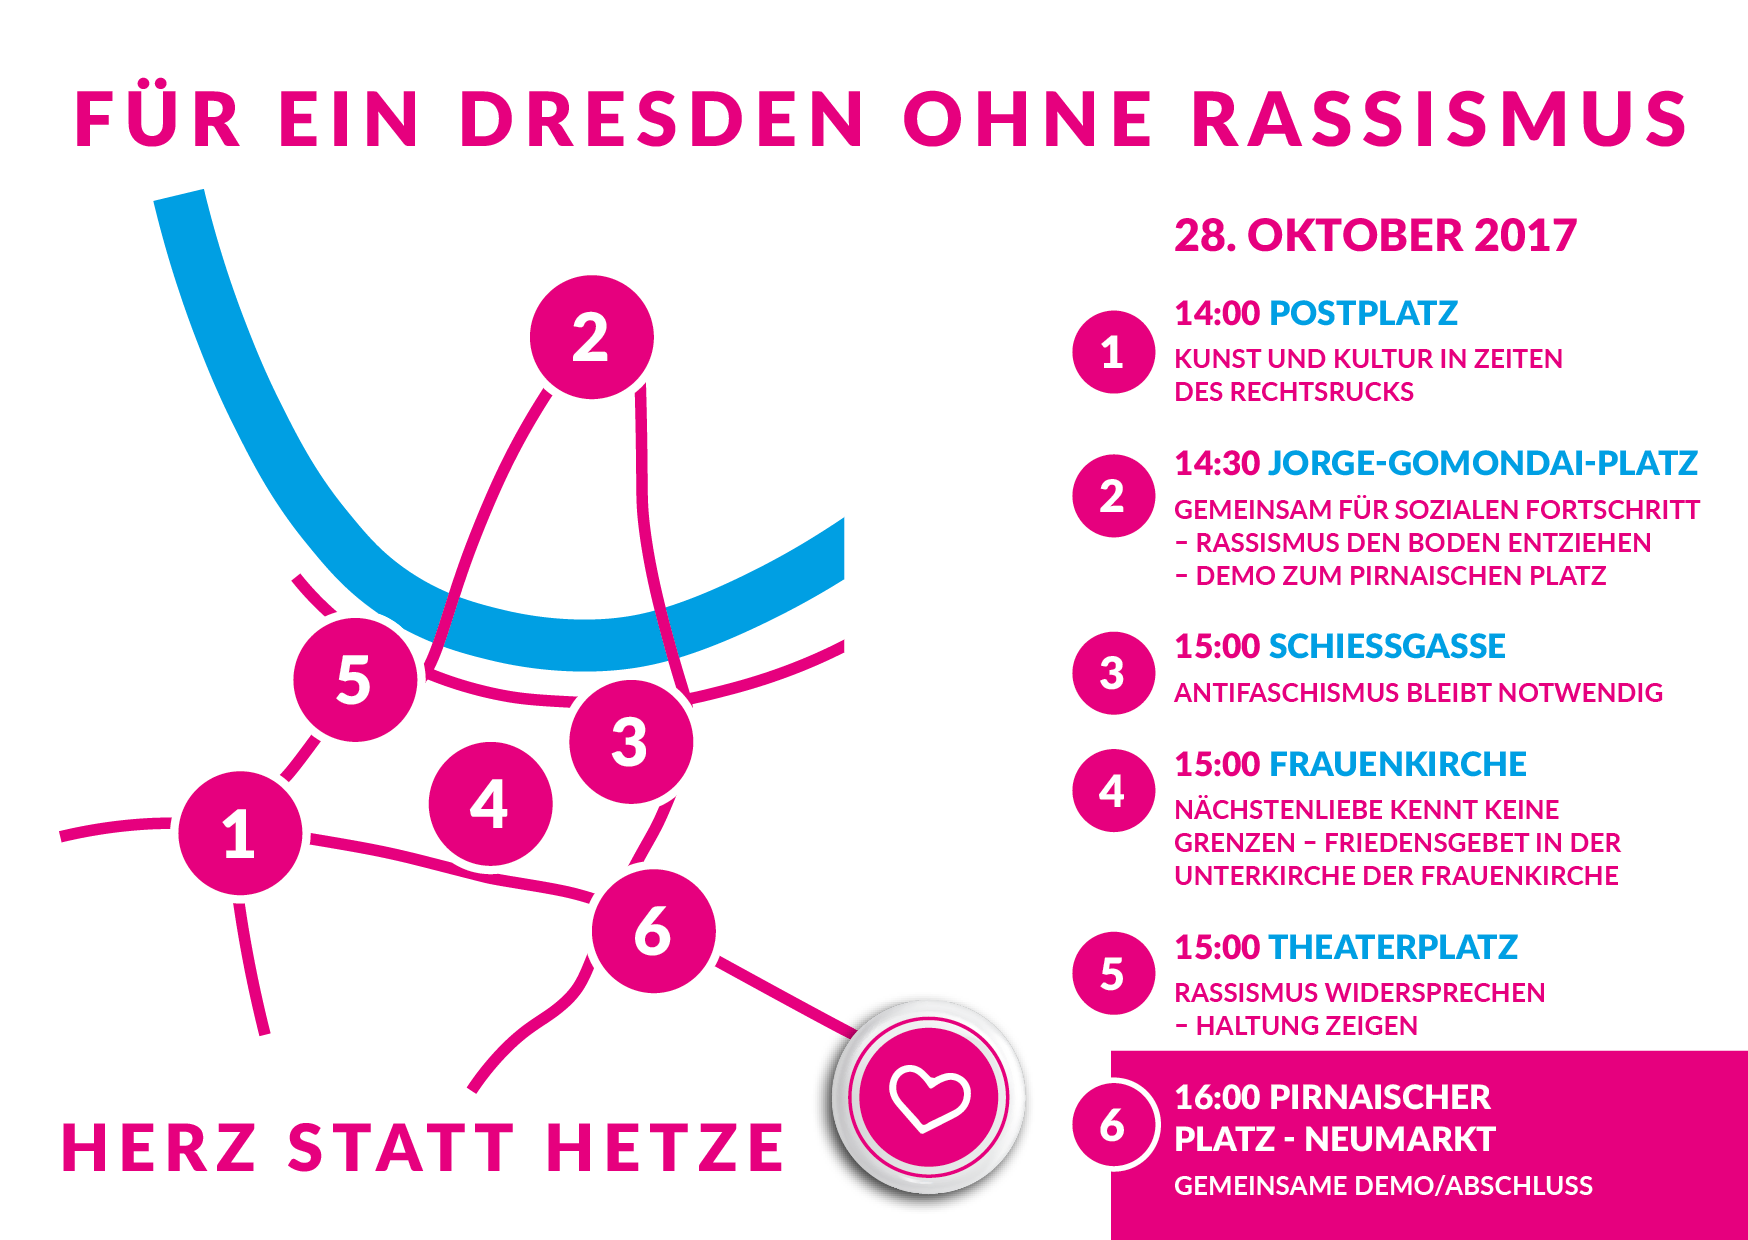
\includegraphics[width=10cm]{images/herz}
% \hfill~
% \rotatebox{90}{\tiny Randall Munroe, \url{http://xkcd.com/208/}, CC-BY-NC 2.5}

\end{frame}

\sectionSlideNoHandout{Rückblick}

\begin{frame}[fragile]\frametitle{Darstellungen von Typ-3-Sprachen}

\begin{tikzpicture}[
	decoration=penciline, decorate,
	node distance = 7mm and 9mm,
	mybox/.style args = {#1/#2}{
		draw=#1,% line color
		fill=#2,% fill color
% 		rounded corners,
		thick,
		text width=26mm, minimum height=12mm, inner sep=1mm, 
		align=flush center
	},
	myboxlabel/.style args = {}{
		draw=devilscss,% line color
		fill=strongyellow!40,% fill color
% 		rounded corners,
		thick,
		text width=21mm, minimum height=10mm, inner sep=1.5mm, 
		align=flush center
	},
	myarrow/.style args = {#1}{
		line width=0.8mm,
		draw=#1,%line color
		%-{Triangle[length=2.8mm,width=4mm,fill=#1]},
		->,
		shorten >=0.5mm, shorten <=0.1mm
	}
]
\pgfmathsetseed{7729}
% \draw[help lines] (0,0) grid (5,5);
\node (reg) [decorate,mybox=black/cyan!40] at (3,-0.6) {reguläre Grammatik};
\node (dfa) [decorate,mybox=black/cyan!40] at (0,-4) {DFA};
\node (nfa) [decorate,mybox=black/cyan!40] at (6,-4) {NFA};
%
\path[myarrow=devilscss,bend left=20](dfa) edge (reg.180);
\node (dfareglabel) [decorate,myboxlabel=,text width=19mm] at (-0.4,-0.7) {"`$q_1 \stackrel{\Sterm{a}}{\to} q_2$"' $\leadsto$ "`$q_1\to\Sterm{a}q_2$"'};
%
\path[myarrow=devilscss,-,bend left=20](reg.0) edge[->] (nfa);
\node (regnfalabel) [decorate,myboxlabel=] at (7.2,-2.1) {"`$q_1\to\Sterm{a}q_2$"' $\leadsto$ "`$q_1 \stackrel{\Sterm{a}}{\to} q_2$"'};
%
\draw[myarrow=devilscss](dfa.10)--(nfa.170);
\node (dfanfalabel) [decorate,myboxlabel=] at (3,-3.0) {\footnotesize DFAs sind spezielle NFAs};
%
\draw[myarrow=devilscss](nfa.190)--(dfa.350);
\node (nfadfalabel) [decorate,myboxlabel=] at (3,-5.0) {\footnotesize Potenzmengen\-konstruktion};
%
\node (sd) [decorate,mybox=black/cyan!40,text width=14mm, minimum height=10mm] at (6,-6.5) {\footnotesize Syntax\-diagramm};
\draw[myarrow=devilscss,<->](sd)--(nfa);
\node (sdnfalabel) [decorate,myboxlabel=, minimum height=0mm,inner sep=1.0mm,text width=10mm] at (6.9,-5.3) {\footnotesize dualer Graph};
\end{tikzpicture}

\end{frame}


\begin{frame}\frametitle{Automaten mit Wortübergängen}

% Eine weitere Variante endlicher Automaten:

\defbox{
Ein \redalert{nichtdeterministischer endlicher Automat mit Wortübergängen} 
\Smach{M} ist ein Tupel $\Smach{M}=\tuple{Q,\Sigma,\Delta,Q_0,F}$ mit
den folgenden Teilen:
\begin{itemize}
\item \textcolor{devilscss}{$Q$: endliche Menge von Zuständen}
\item \textcolor{devilscss}{$\Sigma$: Alphabet}
\item $\Delta$: Übergangsrelation, eine \alert{endliche} Relation $\Delta\subseteq Q\times\Sigma^* \times Q$
\item \textcolor{devilscss}{$Q_0$: Menge möglicher {Startzustände} $Q_0\subseteq Q$}
\item \textcolor{devilscss}{$F$: Menge von {Endzuständen} $F\subseteq Q$}
\end{itemize}
}
Die Sprache solcher Automaten wird wie bei NFAs definiert, nur dass in
einem Schritt beliebige Wörter gelesen werden können.

\pause

\doodlebox{darkgreen}{%
Beispiel:\hspace{-5mm}
\begin{tikzpicture}[baseline={([yshift=-2ex]current bounding box.north)}]
% \draw[help lines] (0,0) grid (7,2);
\node (s1) [circle,draw=black,thick] at (0,0) {$q_0$};
\node (s2) [circle,draw=black,thick] at (1.5,0) {$q_1$};
\node (s3) [circle,draw=black,thick] at (1.5,1.4) {$q_2$};
\node (s4) [double,circle,draw=black,thick] at (0,1.4) {$q_3$};
%
\path[->,line width=0.5mm](-1,0) edge (s1);
\path[->,line width=0.5mm](s1) edge [loop above] node[left] {\Sterm{na}} (s1);
% \path[->,line width=0.5mm](s2) edge [loop above] node[right] {\Sterm{bb}} (s2);
\path[->,line width=0.5mm](s1) edge node[above] {$\epsilon$} (s2);
\path[->,line width=0.5mm](s2) edge node[right] {\Sterm{ba}} (s3);
\path[->,line width=0.5mm](s3) edge node[above] {\Sterm{tman}} (s4);
\end{tikzpicture}%
\hspace{3mm}
\begin{minipage}[t]{5.7cm}
$\Delta = \{\tuple{q_0,\Sterm{na},q_0}, \tuple{q_0,\epsilon,q_1}, \tuple{q_1,\Sterm{ba},q_2},$\\ $\tuple{q_2,\Sterm{tman},q_3}\}$\\[1ex]
Akzeptierte Sprache\only<2>{?}\visible<3->{:}\\
\visible<3->{$\{\Sterm{na}\}^* \circ \{\Sterm{batman}\}$}
\end{minipage}
}

\end{frame}


\begin{frame}\frametitle{Wortübergänge machen NFAs nicht stärker}

\theobox{Satz: Jede von einem NFA mit Wortübergängen akzeptierte Sprache, wird auch von einem normalen NFA akzeptiert.}
\pause

\emph{Beweis:} Wir eliminieren zunächst Wortübergänge für Wörter $w\neq\epsilon$.\medskip
\pause

Für jeden Übergang $q\stackrel{w}{\to}q'$ mit $w=\Sterm{a_1}\cdots \Sterm{a_n}$ und $n\geq 2$:\\
\begin{itemize}
\item Führe $n-1$ neue Zustände $p_1,\ldots,p_{n-1}$ ein.
\item Ersetze $q\stackrel{w}{\to}q'$ durch Übergänge $q\stackrel{\Sterm{a_1}}{\to}p_1$, $p_1\stackrel{\Sterm{a_2}}{\to}p_2$, \ldots, \ghost{$p_{n-1}\stackrel{\Sterm{a_n}}{\to}q'$.}
\end{itemize}
Es ist leicht zu sehen, dass diese Umformung korrekt ist.
\bigskip

Dadurch erhalten wir einen NFA, in dem nur noch zwei Formen von Übergängen vorkommen:
$q_1\stackrel{\Sterm{a}}{\to}q_2$ und $q_1\stackrel{\epsilon}{\to}q_2$.

\end{frame}

\begin{frame}\frametitle{$\epsilon$-Übergänge machen NFA nicht stärker}

\defbox{Ein NFA mit Wortübergängen, bei dem alle Übergänge die Form
$q_1\stackrel{\Sterm{a}}{\to}q_2$ oder $q_1\stackrel{\epsilon}{\to}q_2$ haben, wird
\redalert{$\epsilon$-NFA} genannt.
}

Um den vorigen Beweis abzuschließen müssen wir noch zeigen:

\theobox{Satz: Jede von einem $\epsilon$-NFA akzeptierte Sprache, wird auch von einem normalen NFA akzeptiert.}\pause

\emph{Beweis:} Sei $\epstrastar$ der reflexive, transitive Abschluss von $\stackrel{\epsilon}{\to}$, d.h. die Menge aller Zustandspaare $\tuple{q,q'}\in Q^2$ für die es Übergänge $q=p_0\stackrel{\epsilon}{\to} p_1\stackrel{\epsilon}{\to}\ldots\stackrel{\epsilon}{\to}p_n=q'$ gibt, mit $n\geq 0$.
\medskip\pause

Für einen $\epsilon$-NFA $\Smach{M}=\tuple{Q,\Sigma,\Delta,Q_0,F}$ definieren wir einen NFA
$\Smach{M}'=\tuple{Q,\Sigma,\delta,Q_0',F}$ wobei
\begin{itemize}
\item $\delta(q,\Sterm{a})=\{ q'\mid q\stackrel{\Sterm{a}}{\to}r\epstrastar q'\text{ für ein }r\in Q\}$
\item $Q_0'=\{q\mid q_0\epstrastar q\text{ für ein }q_0\in Q\}$
\end{itemize}
Wir behaupten $\Slang{L}(\Smach{M})=\Slang{L}(\Smach{M}')$.

% Eliminierung mit transitiver Hülle der eps Transitionen
\end{frame}

\begin{frame}\frametitle{Beispiel: Eliminierung von Wortübergängen}

\begin{tikzpicture}[baseline={(current bounding box.center)}]
% \draw[help lines] (0,0) grid (7,2);
\node (s1) [circle,draw=black,thick] at (0,0) {$q_0$};
\node (s2) [circle,draw=black,thick] at (1.5,0) {$q_1$};
\node (s3) [circle,draw=black,thick] at (1.5,1.4) {$q_2$};
\node (s4) [double,circle,draw=black,thick] at (0,1.4) {$q_3$};
%
\path[->,line width=0.5mm](-1,0) edge (s1);
\path[->,line width=0.5mm,onslide={<3>{dashed,darkred}}](s1) edge [loop above] node[left] {\Sterm{na}} (s1);
% \path[->,line width=0.5mm](s2) edge [loop above] node[right] {\Sterm{bb}} (s2);
\path[->,line width=0.5mm](s1) edge node[above] {$\epsilon$} (s2);
\path[->,line width=0.5mm,onslide={<4>{dashed,darkred}}](s2) edge node[right] {\Sterm{ba}} (s3);
\path[->,line width=0.5mm,onslide={<5>{dashed,darkred}}](s3) edge node[above] {\Sterm{tman}} (s4);
\end{tikzpicture}%
\hspace{1cm}
% 
\onslide<2->{%
\begin{tikzpicture}[baseline={([yshift=-2ex]current bounding box.center)}]
% \draw[help lines] (0,0) grid (7,2);
\node (s1) [circle,draw=black,thick] at (0,0) {$q_0$};
\node (s2) [circle,draw=black,thick] at (3,0) {$q_1$};
\node (s3) [circle,draw=black,thick] at (3,3) {$q_2$};
\node (s4) [double,circle,draw=black,thick] at (0,3) {$q_3$};
%
% \path[->,line width=0.5mm](s2) edge node[right] {\Sterm{ba}} (s3);
\onslide<4->{\node (p1) [circle,draw=black,thick] at (3,1.5) {$p_2$};
\path[->,line width=0.5mm](s2) edge node[right] {\Sterm{b}} (p1);
\path[->,line width=0.5mm](p1) edge node[right] {\Sterm{a}} (s3);}
% \path[->,line width=0.5mm](s1) edge [loop above] node[left] {\Sterm{na}} (s1);
\onslide<3->{\node (p5) [circle,draw=black,thick] at (0,1.5) {$p_1$};
\path[->,line width=0.5mm,bend left](s1) edge node[left] {\Sterm{n}} (p5);
\path[->,line width=0.5mm,bend left,onslide={<7>{dashed,darkred}}](p5) edge node[right] {\Sterm{a}} (s1);}
% \path[->,line width=0.5mm](s3) edge node[above] {\Sterm{tman}} (s4);
\onslide<5->{\node (p2) [circle,draw=black,thick] at (3,4.5) {$p_3$};
\node (p3) [circle,draw=black,thick] at (1.5,4.5) {$p_4$};
\node (p4) [circle,draw=black,thick] at (0,4.5) {$p_5$};
\path[->,line width=0.5mm](s3) edge node[right] {\Sterm{t}} (p2);
\path[->,line width=0.5mm](p2) edge node[above] {\Sterm{m}} (p3);
\path[->,line width=0.5mm](p3) edge node[above] {\Sterm{a}} (p4);
\path[->,line width=0.5mm](p4) edge node[right] {\Sterm{n}} (s4);}
%
\path[->,line width=0.5mm,onslide={<6>{dashed,darkred}}](-1,0) edge (s1);
\onslide<6->{\path[->,line width=0.5mm](3,-1) edge (s2);}
\path[->,line width=0.5mm,devilscss,dotted,onslide={<6,7>{dashed,darkred}}](s1) edge node[above] {$\epsilon$} (s2);
\onslide<7->{\path[->,line width=0.5mm](p5) edge node[above] {\Sterm{a}} (s2);}
%
\onslide<8->{\node (crossmark) at (1.5,0) {\Huge$\textcolor{darkred}{\boldsymbol{\times}}$};}
\end{tikzpicture}}%

\ghost{\raisebox{0mm}{\hspace{3.0cm}\onslide<6-8>{$\epstrastar = \{\tuple{q_0,q_1}\}\cup\{\tuple{q,q}\mid q\in Q\}$}}}

\end{frame}

\begin{frame}[t]\frametitle{Korrektheit $\epsilon$-NFA $\leadsto$ NFA (1)}
% beide Richtungen einzeln, durch Abbildung der Läufe

Wir behaupten $\Slang{L}(\Smach{M})=\Slang{L}(\Smach{M}')$.\\[1ex]

\emph{Beweis:} Richtung $\Slang{L}(\Smach{M})\supseteq\Slang{L}(\Smach{M}')$.\pause

\begin{itemize}
\item Sei $w=\Sterm{a_1}\cdots\Sterm{a_n}\in \Slang{L}(\Smach{M'})$ und $p_0p_1\ldots p_n$ ein akzeptierender Lauf für $w$ in $\Smach{M'}$\pause
\item Dann gibt es in $\Smach{M}'$ Übergänge:
\[ p_0\stackrel{\Sterm{a_1}}{\to}p_1\stackrel{\Sterm{a_2}}{\to}\ldots\stackrel{\Sterm{a_n}}{\to}p_n\]\pause
\item Dann gilt in $\Smach{M}$:
\[ q_0\epstrastar p_0\stackrel{\Sterm{a_1}}{\to}q_1\epstrastar p_1\stackrel{\Sterm{a_2}}{\to}\ldots\stackrel{\Sterm{a_n}}{\to}q_n\epstrastar p_n\]\pause
\item Es ist $q_0\in Q_0$ (da $p_0\in Q_0'$) und $p_n\in F$, also hat $\Smach{M}$ einen akzeptierenden Lauf der Form $q_0\ldots p_0q_1\ldots p_1\ldots q_n\ldots p_n$.\pause
\end{itemize}
Also ist $w\in\Slang{L}(\Smach{M})$.

\end{frame}

\begin{frame}[t]\frametitle{Korrektheit $\epsilon$-NFA $\leadsto$ NFA (2)}
% beide Richtungen einzeln, durch Abbildung der Läufe

Wir behaupten $\Slang{L}(\Smach{M})=\Slang{L}(\Smach{M}')$.\\[1ex]

\emph{Beweis:} Richtung $\Slang{L}(\Smach{M})\subseteq\Slang{L}(\Smach{M}')$.\pause

\begin{itemize}
\item Sei $w=\Sterm{a_1}\cdots\Sterm{a_n}\in \Slang{L}(\Smach{M})$.
\item Dann gibt es einen akzeptierenden Lauf mit Übergängen der Form
\[ q_0\epstrastar p_0\stackrel{\Sterm{a_1}}{\to}q_1\epstrastar p_1\stackrel{\Sterm{a_2}}{\to}\ldots\stackrel{\Sterm{a_n}}{\to}q_n\epstrastar p_n\]\pause
\item Dann gibt es in $\Smach{M}'$ Übergänge:
\[ p_0\stackrel{\Sterm{a_1}}{\to}p_1\stackrel{\Sterm{a_2}}{\to}\ldots\stackrel{\Sterm{a_n}}{\to}p_n\]
\item Dies führt zu einem akzeptierenden Lauf in $\Smach{M}'$.
\end{itemize}
Also ist $w\in\Slang{L}(\Smach{M}')$.\qed

\end{frame}

\begin{frame}\frametitle{$\epsilon$-NFA: Variationen}
% Anmerkung zur Variation im Beweis, speziell bezüglich beidseitiger esp Eliminierung (wie bei FB)

Die Konstruktion im Beweis "`verlängert"' normale Übergänge "`nach rechts"' durch Anhängen von $\epsilon$-Transitionen.
\medskip

\narrowcentering{%
\scalebox{0.7}{%
\begin{tikzpicture}[baseline={(current bounding box.center)}]
% \draw[help lines] (0,0) grid (7,2);
\node (s1) [circle,draw=black,thick] at (0,0) {$q_0$};
\node (s2) [circle,draw=black,thick] at (2,0) {$q_1$};
\node (s3) [circle,draw=black,thick] at (4,0) {$q_2$};
\node (s4) [double,circle,draw=black,thick] at (6,0) {$q_3$};
%
\path[->,line width=0.5mm](0,-0.8) edge (s1);
\path[->,line width=0.5mm](s1) edge node[above] {$\epsilon$} (s2);
\path[->,line width=0.5mm](s2) edge node[above] {$\Sterm{a}$} (s3);
\path[->,line width=0.5mm](s3) edge node[above] {$\epsilon$} (s4);
%
\path[->,line width=0.5mm,darkred,dotted](2,-0.8) edge (s2);
\path[->,line width=0.5mm, bend right,darkred,dotted](s2) edge node[above,yshift=-2pt] {$\Sterm{a}$} (s4);
% \path[->,line width=0.5mm, bend right](s1) edge node[above,yshift=-2pt] {$\Sterm{a}$} (s3);
% \path[->,line width=0.5mm, bend right=40](s1) edge node[above,yshift=-2pt] {$\Sterm{a}$} (s4);
\end{tikzpicture}}}
\bigskip\pause

Man kann alternative Konstruktionen für den Beweis angeben:
\begin{itemize}
\item \alert{"`Verlängerung nach links"':} $\epsilon$-Transitionen vor normalen Übergängen; Anfangszustände werden beibehalten; dafür werden Endzustände mit $\epsilon$-Transitionen erweitert\medskip

\narrowcentering{%
\scalebox{0.7}{%
\begin{tikzpicture}[baseline={(current bounding box.center)}]
% \draw[help lines] (0,0) grid (7,2);
\node (s1) [circle,draw=black,thick] at (0,0) {$q_0$};
\node (s2) [circle,draw=black,thick] at (2,0) {$q_1$};
\node (s3) [double,circle,draw=darkred,thick] at (4,0) {$q_2$};
\node (s4) [double,circle,draw=black,thick] at (6,0) {$q_3$};
%
\path[->,line width=0.5mm](0,-0.8) edge (s1);
\path[->,line width=0.5mm](s1) edge node[above] {$\epsilon$} (s2);
\path[->,line width=0.5mm](s2) edge node[above] {$\Sterm{a}$} (s3);
\path[->,line width=0.5mm](s3) edge node[above] {$\epsilon$} (s4);
%
% \path[->,line width=0.5mm, bend right](s2) edge node[above,yshift=-2pt] {$\Sterm{a}$} (s4);
\path[->,line width=0.5mm, bend right,darkred,dotted](s1) edge node[above,yshift=-2pt] {$\Sterm{a}$} (s3);
% \path[->,line width=0.5mm, bend right=40](s1) edge node[above,yshift=-2pt] {$\Sterm{a}$} (s4);
\end{tikzpicture}}}
\item \alert{"`Verlängerung in beide Richtungen"':} $\epsilon$-Transitionen vor und nach normalen Übergängen; Anfangs- und Endzustände können beibehalten werden$^*$
% \hspace{3cm}\ghost{\raisebox{-1cm}{\begin{minipage}{3cm}
% {\baselineskip=0.2ex \lineskip=0pt.\medskip
% \end{minipage}}}

\narrowcentering{%
\scalebox{0.7}{%
\begin{tikzpicture}[baseline={(current bounding box.center)}]
% \draw[help lines] (0,0) grid (7,2);
\node (s1) [circle,draw=black,thick] at (0,0) {$q_0$};
\node (s2) [circle,draw=black,thick] at (2,0) {$q_1$};
\node (s3) [circle,draw=black,thick] at (4,0) {$q_2$};
\node (s4) [double,circle,draw=black,thick] at (6,0) {$q_3$};
%
\path[->,line width=0.5mm](0,-0.8) edge (s1);
\path[->,line width=0.5mm](s1) edge node[above] {$\epsilon$} (s2);
\path[->,line width=0.5mm](s2) edge node[above] {$\Sterm{a}$} (s3);
\path[->,line width=0.5mm](s3) edge node[above] {$\epsilon$} (s4);
%
\path[->,line width=0.5mm, bend right,darkred,dotted](s2) edge node[above,yshift=-2pt] {$\Sterm{a}$} (s4);
\path[->,line width=0.5mm, bend right,darkred,dotted](s1) edge node[above,yshift=-2pt] {$\Sterm{a}$} (s3);
\path[->,line width=0.5mm, bend right=35,darkred,dotted](s1) edge node[above,yshift=-2pt] {$\Sterm{a}$} (s4);
\end{tikzpicture}}}\\[-1ex]
{\tiny *) Ausnahme: Anfangszustände mit $\epsilon$-Pfad zu einem Endzustand werden Endzustand}
\end{itemize}

\end{frame}

\sectionSlide{Abschlusseigenschaften}

\newcommand{\mytabnote}[2]{\ghost{#1}\hspace{2cm}{\textcolor{devilscss}{(#2)}}}
\newcommand{\myhitabnote}[2]{\ghost{#1}\hspace{2cm}{\textcolor{darkred}{#2}}}
\begin{frame}\frametitle{Abschlusseigenschaften regulärer Sprachen}

Reguläre Sprachen sind unter zahlreichen Operationen abgeschlossen:

\theobox{
Satz: Wenn $\Slang{L}$, $\Slangsub{L}{1}$ und $\Slangsub{L}{2}$ reguläre Sprachen sind, dann beschreiben auch die
folgenden Ausdrücke reguläre Sprachen:
\begin{enumerate}[(1)]
\item \mytabnote{$\Slangsub{L}{1}\cup\Slangsub{L}{2}$}{Abschluss unter Vereinigung}
\item \mytabnote{$\Slangsub{L}{1}\cap\Slangsub{L}{2}$}{Abschluss unter Schnitt}
\item \mytabnote{$\overline{\Slang{L}}$}{Abschluss unter Komplement}
\item \mytabnote{$\Slangsub{L}{1}\circ\Slangsub{L}{2}$}{Abschluss unter Konkatenation}
\item \mytabnote{$\Slang{L}^*$}{Abschluss unter Kleene-Stern}
\end{enumerate}
}\pause

\emph{Beweisidee:} Für jede Operation auf Sprachen entwickeln wir eine entsprechende
\alert{Operation auf Automaten}. Dadurch konstruieren wir Automaten, welche die
gesuchte Sprache erkennen (daher muss die Sprache regulär sein).

% Satz: Abschluss unter cup cap circ compl *
% Erläuterung
% Beweisplan (via Automaten)

\end{frame}

\begin{frame}\frametitle{Vereinigung von NFAs}
% Operator kann mit cup+ bezeichnet werden

Ein NFA zur Vereinigung von zwei NFAs ist leicht zu finden\pause:

\defbox{Gegeben seien zwei NFAs $\Smach{M}_1=\tuple{Q_1,\Sigma,\delta_1,Q_{0,1},F_1}$ und $\Smach{M}_2=\tuple{Q_2,\Sigma,\delta_2,Q_{0,2},F_2}$ mit $Q_1\cap Q_2=\emptyset$ (o.B.d.A.). 
\medskip

Der \redalert{Vereinigungsautomat $\Smach{M}_1\oplus\Smach{M}_2$} ist
gegeben durch $\tuple{Q_1\cup Q_2,\Sigma,\delta_{12},Q_{0,1}\cup Q_{0,2},F_1\cup F_2}$ wobei\\[1ex]
\narrowcentering{$\delta_{12}(q,\Sterm{a}) = \left\{\begin{array}{lr}
	\delta_1(q,\Sterm{a}) & \text{ falls $q\in Q_1$}\\
	\delta_2(q,\Sterm{a}) & \text{ falls $q\in Q_2$}
\end{array}\right.$}
}\pause

Das folgende Ergebnis ist leicht zu sehen:

\theobox{Satz: $\Slang{L}(\Smach{M}_1\oplus\Smach{M}_2) = \Slang{L}(\Smach{M}_1)\cup\Slang{L}(\Smach{M}_2)$.
}

Also sind reguläre Sprachen unter Vereinigung abgeschlossen.

\end{frame}

\begin{frame}\frametitle{Beispiel}

Die Vereinigung der NFAs\bigskip

{%
\begin{tikzpicture}[baseline={(q1.base)}]
% \draw[help lines] (0,0) grid (7,2);
\node (q1) [circle,draw=black,thick,double] at (0,0) {$q_1$};
\node (q2) [circle,draw=black,thick] at (2,0) {$q_2$};
\node (q3) [circle,draw=black,thick,double] at (4,0) {$q_3$};
%
\path[->,line width=0.5mm](0,1) edge (q1);
\path[->,line width=0.5mm](q1) edge node[above] {\Sterm{1}} (q2);
\path[->,line width=0.5mm, bend left](q2) edge node[above] {\Sterm{0}} (q3);
\path[->,line width=0.5mm, bend left](q3) edge node[above] {\Sterm{1}} (q2);
\end{tikzpicture}
\hfill und\hfill 
\begin{tikzpicture}[baseline={(p1.base)}]
% \draw[help lines] (0,0) grid (7,2);
\node (p1) [circle,draw=black,thick] at (0,0) {$p_1$};
\node (p2) [circle,draw=black,thick,double] at (2,0) {$p_2$};
%
\path[->,line width=0.5mm](0,1) edge (p1);
\path[->,line width=0.5mm, bend left](p1) edge node[above] {\Sterm{0}} (p2);
\path[->,line width=0.5mm, bend left](p2) edge node[above] {\Sterm{1}} (p1);
\end{tikzpicture}
}\bigskip

ergibt den NFA \ldots\pause\bigskip

{%
\begin{tikzpicture}[baseline={(q1.base)}]
% \draw[help lines] (0,0) grid (7,2);
\node (q1) [circle,draw=black,thick,double] at (0,0) {$q_1$};
\node (q2) [circle,draw=black,thick] at (2,0) {$q_2$};
\node (q3) [circle,draw=black,thick,double] at (4,0) {$q_3$};
%
\path[->,line width=0.5mm](0,1) edge (q1);
\path[->,line width=0.5mm](q1) edge node[above] {\Sterm{1}} (q2);
\path[->,line width=0.5mm, bend left](q2) edge node[above] {\Sterm{0}} (q3);
\path[->,line width=0.5mm, bend left](q3) edge node[above] {\Sterm{1}} (q2);
\end{tikzpicture}
\hfill 
\begin{tikzpicture}[baseline={(p1.base)}]
% \draw[help lines] (0,0) grid (7,2);
\node (p1) [circle,draw=black,thick] at (0,0) {$p_1$};
\node (p2) [circle,draw=black,thick,double] at (2,0) {$p_2$};
%
\path[->,line width=0.5mm](0,1) edge (p1);
\path[->,line width=0.5mm, bend left](p1) edge node[above] {\Sterm{0}} (p2);
\path[->,line width=0.5mm, bend left](p2) edge node[above] {\Sterm{1}} (p1);
\end{tikzpicture}
}\bigskip

\pause{}Akzeptierte Sprache: $\{\Sterm{1}\Sterm{0}\}^*\cup (\{\Sterm{0}\Sterm{1}\}^*\circ\{\Sterm{0}\})=
\{\epsilon,\Sterm{0}\} \circ \{\Sterm{1}\Sterm{0}\}^* $

\end{frame}

\begin{frame}\frametitle{Abschluss unter Schnitt}

\theobox{
Satz: Wenn $\Slang{L}$, $\Slangsub{L}{1}$ und $\Slangsub{L}{2}$ reguläre Sprachen sind, dann beschreiben auch die
folgenden Ausdrücke reguläre Sprachen:
\begin{enumerate}[(1)]
\item \mytabnote{$\Slangsub{L}{1}\cup\Slangsub{L}{2}$}{Abschluss unter Vereinigung}
\item \myhitabnote{$\Slangsub{L}{1}\cap\Slangsub{L}{2}$}{Abschluss unter Schnitt}
\item \mytabnote{$\overline{\Slang{L}}$}{Abschluss unter Komplement}
\item \mytabnote{$\Slangsub{L}{1}\circ\Slangsub{L}{2}$}{Abschluss unter Konkatenation}
\item \mytabnote{$\Slang{L}^*$}{Abschluss unter Kleene-Stern}
\end{enumerate}
}

\end{frame}

\begin{frame}\frametitle{Schnitte mit Automaten}
% Ziel und Idee angeben

\alert{Gegeben:} Automaten $\Smach{M}_1$ und $\Smach{M}_2$\\[1ex]
\alert{Gesucht:} Automat $\Smach{M}$ mit $\Slang{L}(\Smach{M})=\Slang{L}(\Smach{M}_1)\cap\Slang{L}(\Smach{M}_2)$
\bigskip

\emph{Idee:}
\begin{itemize}
\item Verarbeite Eingabe gleichzeitig synchron auf beiden Automaten
\item Akzeptiere, wenn beide Automaten akzeptieren
\end{itemize}
$\leadsto$ \alert{Produktautomat}

\end{frame}

\begin{frame}\frametitle{Der Produktautomat}
% Einfuehren fuer NFAs
% Notation koennte umkreistes \times verwenden
% Anschliessend beobachten, dass das auch fuer DFAs geht

\emph{Erinnerung:} Gegeben Mengen $A$ und $B$ bezeichnet $A\times B$ die Menge aller möglichen Paare von Elementen aus $A$ und $B$, d.h. $A\times B=\{\tuple{a,b}\mid a\in A, b\in B\}$.
\medskip

\defbox{Gegeben seien zwei NFAs $\Smach{M}_1=\tuple{Q_1,\Sigma,\delta_1,Q_{0,1},F_1}$ und $\Smach{M}_2=\tuple{Q_2,\Sigma,\delta_2,Q_{0,2},F_2}$. 
\medskip

Der \redalert{Produktautomat $\Smach{M}_1\otimes\Smach{M}_2$} ist
gegeben durch $\tuple{Q_1\times Q_2,\Sigma,\delta,Q_{0,1}\times Q_{0,2},F_1\times F_2}$ wobei\\[1ex]
\narrowcentering{$\delta(\tuple{q_1,q_2},\Sterm{a}) =\delta_1(q_1,\Sterm{a})\times\delta_2(q_2,\Sterm{a})$}
}\pause

Wir werden zeigen, dass dies der gesuchte Automat ist:

\theobox{Satz: $\Slang{L}(\Smach{M}_1\otimes\Smach{M}_2) = \Slang{L}(\Smach{M}_1)\cap\Slang{L}(\Smach{M}_2)$.
}

Also sind reguläre Sprachen unter Schnitten abgeschlossen.
\bigskip

\emph{Beobachtung:} Wenn $|A|=|B|=1$, dann ist $|A\times B|=1$. Also ist der Produktautomat von DFAs ebenfalls ein DFA.

\end{frame}

\begin{frame}[t]\frametitle{Beispiel}

\narrowcentering{%
\begin{tikzpicture}[baseline={(a.base)}]
% \draw[help lines] (0,0) grid (7,2);
\node (a) [circle,draw=black,thick,double,onslide={<5>{fill=strongyellow}}] at (0,0) {$A$};
\node (b) [circle,draw=black,thick] at (3,0) {$B$};
%
\path[->,line width=0.5mm,onslide={<4>{dashed,darkred}}](0,1) edge (a);
\path[->,line width=0.5mm, bend left,onslide={<6,8>{dashed,darkred}}](a) edge node[above] {\Sterm{0}} (b);
\path[->,line width=0.5mm, bend left,onslide={<10,12>{dashed,darkred}}](b) edge node[above] {\Sterm{0}} (a);
\path[->,line width=0.5mm,onslide={<7,9>{dashed,darkred}}](a) edge [loop below] node[below] {\Sterm{1}} (a);
\path[->,line width=0.5mm,onslide={<11,13>{dashed,darkred}}](b) edge [loop below] node[below] {\Sterm{1}} (b);
% ,onslide={<7>{dashed,darkred}}
\end{tikzpicture}
%
\hfill
%
\begin{tikzpicture}[baseline={(current bounding box.center)}]
% \draw[help lines] (0,0) grid (7,2);
\node (c) [circle,draw=black,thick] at (0,0) {$C$};
\node (d) [circle,draw=black,thick,double,onslide={<5>{fill=strongyellow}}] at (0,-2) {$D$};
%
\path[->,line width=0.5mm,onslide={<4>{dashed,darkred}}](-1,0) edge (c);
\path[->,line width=0.5mm,onslide={<4>{dashed,darkred}}](-1,-2) edge (d);
\path[->,line width=0.5mm,onslide={<6,7,10,11>{dashed,darkred}}](c) edge node[right] {\Sterm{0}, \Sterm{1}} (d);
\path[->,line width=0.5mm,onslide={<6,10>{dashed,darkred}}](c) edge [loop right] node[right] {\Sterm{0}} (c);
\path[->,line width=0.5mm,onslide={<9,13>{dashed,darkred}}](d) edge [loop right] node[right] {\Sterm{1}} (d);
% ,onslide={<7>{dashed,darkred}}
\end{tikzpicture}}

\onslide<1>{\narrowcentering{Sprachen?}}

\onslide<2->{\narrowcentering{"`Wörter mit gerader Anzahl \Sterm{0}"'\hfill "`Wörter ohne Infix \Sterm{10}"'}}
\bigskip

\onslide<3->{%
\narrowcentering{%
\begin{tikzpicture}[baseline={(current bounding box.center)}]
% \draw[help lines] (0,0) grid (7,2);
\node (ac) [circle,draw=black,thick] at (0,0) {$\tuple{A,C}$};
\node (ad) [circle,draw=black,thick,onslideprint={<5->{double}},onslide={<5>{fill=strongyellow}}] at (0,-2) {$\tuple{A,D}$};
\node (bc) [circle,draw=black,thick] at (3,0) {$\tuple{B,C}$};
\node (bd) [circle,draw=black,thick] at (3,-2) {$\tuple{B,D}$};
%
\onslide<4->{\path[->,line width=0.5mm,onslide={<4>{dashed,darkred}}](-1,1) edge (ac);}
\onslide<4->{\path[->,line width=0.5mm,onslide={<4>{dashed,darkred}}](-1,-1) edge (ad);}
\onslide<6->{\path[->,line width=0.5mm, bend left,onslide={<6>{dashed,darkred}}](ac) edge node[above] {\Sterm{0}} (bc);}
\onslide<10->{\path[->,line width=0.5mm, bend left,onslide={<10>{dashed,darkred}}](bc) edge node[above] {\Sterm{0}} (ac);}
%
\onslide<10->{\path[->,line width=0.5mm,onslide={<10>{dashed,darkred}}](bc.240) edge node[below,xshift=7mm,yshift=3mm] {\Sterm{0}} (ad.35);}
\onslide<11->{\path[->,line width=0.5mm,onslide={<11>{dashed,darkred}}](bc) edge node[right] {\Sterm{1}} (bd);}
\onslide<6->{
\path[-,line width=1.1mm,white,shorten >=3mm,shorten <=3mm](ac.300) edge (bd.135);
\path[->,line width=0.5mm,onslide={<6>{dashed,darkred}}](ac.300) edge node[below,xshift=-7mm,yshift=3mm] {\Sterm{0}} (bd.135);
}
\onslide<7->{\path[->,line width=0.5mm,onslide={<7>{dashed,darkred}}](ac) edge node[right] {\Sterm{1}} (ad);}
%
\onslide<13-14>{\path[->,line width=0.5mm,onslide={<13>{dashed,darkred}}](bd) edge [loop right] node[right] {\Sterm{1}} (bd);}
\onslide<9->{\path[->,line width=0.5mm,onslide={<9>{dashed,darkred}}](ad) edge [loop right] node[right] {\Sterm{1}} (ad);}
% ,onslide={<7>{dashed,darkred}}
\end{tikzpicture}}}

\end{frame}

\begin{frame}\frametitle{Beweis der Korrektheit des Produktautomaten}

"`$\Slang{L}(\Smach{M}_1\otimes\Smach{M}_2) \subseteq \Slang{L}(\Smach{M}_1)\cap\Slang{L}(\Smach{M}_2)$"'~~ Sei $w=\Sterm{a_1}\cdots\Sterm{a_n}\in\Slang{L}(\Smach{M}_1\otimes\Smach{M}_2)$.\pause
\begin{itemize}
\item Also gibt es einen akzeptierenden Lauf $\tuple{q_1^0,q_2^0}\tuple{q_1^1,q_2^1}\ldots\tuple{q_1^n,q_2^n}$\pause
\item Dann gilt:
\begin{itemize}
\item $\tuple{q_1^0,q_2^0}\in Q_{0,1}\times Q_{0,2}$, also $q_1^0\in Q_{0,1}$ und $q_2^0\in Q_{0,2}$
\item $\tuple{q_1^n,q_2^n}\in F_1\times F_2$, also $q_1^n\in F_1$ und $q_2^n\in F_2$
\item $\tuple{q_1^i,q_2^i}\in \delta(\tuple{q_1^{i-1},q_2^{i-1}},\Sterm{a_i})$,\\ also
$q_1^i\in \delta_1(q_1^{i-1},\Sterm{a_i})$ und $q_2^i\in \delta_2(q_2^{i-1},\Sterm{a_i})$\pause
\end{itemize}
\item Daher sind $q_1^0 q_1^1 \ldots q_1^n$ und $q_2^0 q_2^1 \ldots q_2^n$ akzeptierende Läufe von $\Smach{M}_1$ und $\Smach{M}_1$.\pause
\end{itemize}
Also ist $w\in\Slang{L}(\Smach{M}_1)$ und $w\in\Slang{L}(\Smach{M}_2)$.\pause
\bigskip

"`$\Slang{L}(\Smach{M}_1\otimes\Smach{M}_2) \supseteq \Slang{L}(\Smach{M}_1)\cap\Slang{L}(\Smach{M}_2)$"'~~
Analoge Schlussfolgerungen in entgegengesetzter Richtung.\qed

\end{frame}

\begin{frame}\frametitle{Abschluss unter Komplement}

\theobox{
Satz: Wenn $\Slang{L}$, $\Slangsub{L}{1}$ und $\Slangsub{L}{2}$ reguläre Sprachen sind, dann beschreiben auch die
folgenden Ausdrücke reguläre Sprachen:
\begin{enumerate}[(1)]
\item \mytabnote{$\Slangsub{L}{1}\cup\Slangsub{L}{2}$}{Abschluss unter Vereinigung}
\item \mytabnote{$\Slangsub{L}{1}\cap\Slangsub{L}{2}$}{Abschluss unter Schnitt}
\item \myhitabnote{$\overline{\Slang{L}}$}{Abschluss unter Komplement}
\item \mytabnote{$\Slangsub{L}{1}\circ\Slangsub{L}{2}$}{Abschluss unter Konkatenation}
\item \mytabnote{$\Slang{L}^*$}{Abschluss unter Kleene-Stern}
\end{enumerate}
}

\end{frame}

\begin{frame}\frametitle{Komplementoperator für DFAs}

\emph{Idee:} Wir können DFA komplementieren, indem wir akzeptierende und verwerfende Zustände vertauschen.
\bigskip

\defbox{Für einen DFA $\Smach{M}=\tuple{Q,\Sigma,\delta,q_0,F}$ sei $\overline{\Smach{M}}$ der\\
DFA $\tuple{Q,\Sigma,\delta,q_0,Q\setminus F}$.}
\bigskip\pause


\emph{Beispiel:}\medskip

\narrowcentering{%
\begin{tikzpicture}[baseline={(a.base)}]
% \draw[help lines] (0,0) grid (7,2);
\node (a) [circle,draw=black,thick,double] at (0,0) {$A$};
\node (b) [circle,draw=black,thick] at (3,0) {$B$};
%
\path[->,line width=0.5mm](0,1) edge (a);
\path[->,line width=0.5mm, bend left](a) edge node[above] {\Sterm{0}} (b);
\path[->,line width=0.5mm, bend left](b) edge node[above] {\Sterm{0}} (a);
\path[->,line width=0.5mm](a) edge [loop below] node[below] {\Sterm{1}} (a);
\path[->,line width=0.5mm](b) edge [loop below] node[below] {\Sterm{1}} (b);
% ,onslide={<7>{dashed,darkred}}
\end{tikzpicture}}\hspace{5mm}$\leadsto$\hspace{5mm}%
%
\narrowcentering{%
\begin{tikzpicture}[baseline={(a.base)}]
% \draw[help lines] (0,0) grid (7,2);
\node (a) [circle,draw=black,thick] at (0,0) {$A$};
\node (b) [circle,draw=black,thick,double] at (3,0) {$B$};
%
\path[->,line width=0.5mm](0,1) edge (a);
\path[->,line width=0.5mm, bend left](a) edge node[above] {\Sterm{0}} (b);
\path[->,line width=0.5mm, bend left](b) edge node[above] {\Sterm{0}} (a);
\path[->,line width=0.5mm](a) edge [loop below] node[below] {\Sterm{1}} (a);
\path[->,line width=0.5mm](b) edge [loop below] node[below] {\Sterm{1}} (b);
% ,onslide={<7>{dashed,darkred}}
\end{tikzpicture}}\medskip

"`Wörter mit gerader Anzahl \Sterm{0}"'\hfill"`Wörter mit ungerader Anzahl \Sterm{0}"'

% Idee einfuehren, Beispiel, unzureichenden Beweis angeben bzw. Beweis nutzen um Fehler zu finden (totaler DFA noetig)

\end{frame}

\begin{frame}\frametitle{Korrektheitsbeweis Komplementierung}

\theobox{Satz: Für jeden DFA gilt $\Slang{L}(\overline{\Smach{M}}) = \overline{\Slang{L}(\Smach{M})}$.}\pause

\emph{Beweis:} "`$\Slang{L}(\overline{\Smach{M}}) \subseteq \overline{\Slang{L}(\Smach{M})}$"'~~
Sei $w=\Sterm{a_1}\cdots\Sterm{a_n}\in\Slang{L}(\overline{\Smach{M}})$.\pause
\begin{itemize}
\item Dann gibt es einen akzeptierenden Lauf $q_0q_1\ldots q_n$ für $w$ in $\overline{\Smach{M}}$.\pause
\item Dann ist $q_n\in Q\setminus F$.\pause
\item Dann ist $q_0q_1\ldots q_n$ ein verwerfender Lauf für $w$ in $\Smach{M}$.\pause
\end{itemize}
Also ist $w\notin{\Slang{L}(\Smach{M})}$, d.h. $w\in\overline{\Slang{L}(\Smach{M})}$.\pause
\bigskip

"`$\Slang{L}(\overline{\Smach{M}}) \supseteq \overline{\Slang{L}(\Smach{M})}$"'~~
Sei $w=\Sterm{a_1}\cdots\Sterm{a_n}\in\overline{\Slang{L}(\Smach{M})}$\pause

\begin{itemize}
\item Dann hat $\Smach{M}$ einen verwerfenden Lauf $p_0p_1\ldots p_m$ für $w$\pause
\item Dann ist (1) $p_m\notin F$ oder (2) $m<|w|$\pause
\item In Fall (1) ist $p_0p_1\ldots p_m$ ein akzeptierender Lauf für $w$ in $\overline{\Smach{M}}$\pause
\item In Fall (2) \ldots ?\pause\\
\ldots vielleicht gar kein akzeptierender Lauf für $w$ in $\overline{\Smach{M}}$ \ldots \pause
\end{itemize}

\narrowcentering{\redalert{Der Satz ist falsch!}}

\end{frame}

\begin{frame}\frametitle{Gegenbeispiel}

\narrowcentering{%
\begin{tikzpicture}[baseline={(current bounding box.center)}]
% \draw[help lines] (0,0) grid (7,2);
\node (c) [circle,draw=black,thick] at (0,0) {$C$};
\node (d) [circle,draw=black,thick,double] at (0,-2) {$D$};
%
\path[->,line width=0.5mm](-1,0) edge (c);
\path[->,line width=0.5mm](c) edge node[right] {\Sterm{1}} (d);
\path[->,line width=0.5mm](c) edge [loop right] node[right] {\Sterm{0}} (c);
\path[->,line width=0.5mm](d) edge [loop right] node[right] {\Sterm{1}} (d);
% ,onslide={<7>{dashed,darkred}}
\end{tikzpicture}\hspace{5mm}$\leadsto$\hspace{5mm}%
%
\begin{tikzpicture}[baseline={(current bounding box.center)}]
% \draw[help lines] (0,0) grid (7,2);
\node (c) [circle,draw=black,thick,double] at (0,0) {$C$};
\node (d) [circle,draw=black,thick] at (0,-2) {$D$};
%
\path[->,line width=0.5mm](-1,0) edge (c);
% \path[->,line width=0.5mm](-1,-2) edge (d);
\path[->,line width=0.5mm](c) edge node[right] {\Sterm{1}} (d);
\path[->,line width=0.5mm](c) edge [loop right] node[right] {\Sterm{0}} (c);
\path[->,line width=0.5mm](d) edge [loop right] node[right] {\Sterm{1}} (d);
% ,onslide={<7>{dashed,darkred}}
\end{tikzpicture}}\bigskip


\onslide<2->{\narrowcentering{Wörter der Form $\Sterm{0}^*\Sterm{1}^+$\hfill \onslide<3->{Wörter der Form $\Sterm{0}^*$}}}
\bigskip

\onslide<4->{Das Wort $\Sterm{010}$ zum Beispiel wird von keinem der beiden Automaten erkannt.}
\bigskip

\onslide<4->{\narrowcentering{\alert{$\leadsto$ keine komplementären Sprachen}}}

\end{frame}

\begin{frame}\frametitle{Korrekte Komplementierung}
% Diskussion warum das auch nicht geht, mit Beispiel

\theobox{Satz: Für jeden DFA \alert{mit totaler Übergangsfunktion} gilt $\Slang{L}(\overline{\Smach{M}}) = \overline{\Slang{L}(\Smach{M})}$.}

\emph{Beweis:} Wie vorher für den falschen Satz, aber diesmal kann der Problemfall (2) der Rückrichtung nicht auftreten.
\bigskip

Daraus folgt der Abschluss regulärer Sprachen unter Komplement, da wir jeden DFA mit totalen Übergängen ausstatten können.
\bigskip\pause

\anybox{devilscss}{
\emph{Auch NFAs dürfen nicht direkt komplementiert werden:}
\begin{itemize}
\item DFAs sind NFAs: unser Gegenbeispiel trifft weiterhin zu
\item Selbst NFAs, in denen jeder Zustand für jedes Symbol mindestens einen Folgezustand hat, können nicht so einfach komplementiert werden (Übung: Finden Sie ein Gegenbeispiel)
\end{itemize}
}

\end{frame}


% \begin{frame}\frametitle{Vereinigung von DFAs}
% % Diskussion; zwei Ideen via Determinisierung cup NFA und via DeMorgan
% \end{frame}
% 
% \begin{frame}\frametitle{Vereinigungsoperator für DFAs}
% % direkte Konstruktion als modifiziertes Produkt ueber totalen DFAs
% % Ev. noch eine Folei fuer die Konstruktino mit partiellen DFA,
% %   aber das hat keinen grossen Mehrwert vgl. mit vorheriger Konstruktion totaler DFA
% \end{frame}

\begin{frame}\frametitle{Abschluss unter Konkatenation}

\theobox{
Satz: Wenn $\Slang{L}$, $\Slangsub{L}{1}$ und $\Slangsub{L}{2}$ reguläre Sprachen sind, dann beschreiben auch die
folgenden Ausdrücke reguläre Sprachen:
\begin{enumerate}[(1)]
\item \mytabnote{$\Slangsub{L}{1}\cup\Slangsub{L}{2}$}{Abschluss unter Vereinigung}
\item \mytabnote{$\Slangsub{L}{1}\cap\Slangsub{L}{2}$}{Abschluss unter Schnitt}
\item \mytabnote{$\overline{\Slang{L}}$}{Abschluss unter Komplement}
\item \myhitabnote{$\Slangsub{L}{1}\circ\Slangsub{L}{2}$}{Abschluss unter Konkatenation}
\item \mytabnote{$\Slang{L}^*$}{Abschluss unter Kleene-Stern}
\end{enumerate}
}

\end{frame}


\begin{frame}\frametitle{Konkatenation von NFAs}

\emph{Idee:} Wir können Automaten hintereinander hängen, indem wir von Endzuständen des ersten
zu Startzuständen des zweiten \ghost{wechseln.}\\
$\leadsto$ besonders elegant geht das mit $\epsilon$-Transitionen
\bigskip

\defbox{Gegeben seien zwei NFAs $\Smach{M}_1=\tuple{Q_1,\Sigma,\delta_1,Q_{0,1},F_1}$ und $\Smach{M}_2=\tuple{Q_2,\Sigma,\delta_2,Q_{0,2},F_2}$ mit $Q_1\cap Q_2=\emptyset$ (o.B.d.A.). 
\medskip

Der \redalert{Konkatenationsautomat $\Smach{M}_1\odot\Smach{M}_2$} ist ein $\epsilon$-NFA 
gegeben durch $\tuple{Q_1\cup Q_2,\Sigma,\delta,Q_{0,1},F_2}$ wobei\\[1ex]
\narrowcentering{$\delta(q,\Sterm{a}) = \left\{\begin{array}{l@{~}r}
	\delta_1(q,\Sterm{a}) & \text{ falls $q\in Q_1$}\\
	\delta_2(q,\Sterm{a}) & \text{ falls $q\in Q_2$}
\end{array}\right.$%
\hfill
$\delta(q,\epsilon) = \left\{\begin{array}{l@{~}r}
	Q_{0,2} & \text{ falls $q\in F_1$}\\
	\emptyset & \text{ andernfalls}
\end{array}\right.$}
}
% \bigskip

$\Smach{M}_1\odot\Smach{M}_2$ simuliert also zunächst $\Smach{M}_1$. In jedem Endzustand aus $F_1$ entscheidet
$\Smach{M}_1\odot\Smach{M}_2$ nichtdeterministisch, diese Simulation fortzusetzen oder mit der Simulation von $\Smach{M}_2$ zu beginnen.

\end{frame}

\begin{frame}\frametitle{Beispiel Konkatenation}

\narrowcentering{%
\begin{tikzpicture}[baseline={(a.base)}]
% \draw[help lines] (0,0) grid (7,2);
\node (a) [circle,draw=black,thick,double] at (0,0) {$A$};
\node (b) [circle,draw=black,thick] at (3,0) {$B$};
%
\path[->,line width=0.5mm](0,0.7) edge (a);
\path[->,line width=0.5mm, bend left](a) edge node[above] {\Sterm{0}} (b);
\path[->,line width=0.5mm, bend left](b) edge node[above] {\Sterm{0}} (a);
\path[->,line width=0.5mm](a) edge [loop below] node[below] {\Sterm{1}} (a);
\path[->,line width=0.5mm](b) edge [loop below] node[below] {\Sterm{1}} (b);
% ,onslide={<7>{dashed,darkred}}
\end{tikzpicture}\hspace{10mm}%
\begin{tikzpicture}[baseline={(a.base)}]
% \draw[help lines] (0,0) grid (7,2);
\node (a) [circle,draw=black,thick,double] at (0,0) {$C$};
\node (b) [circle,draw=black,thick] at (3,0) {$D$};
%
\path[->,line width=0.5mm](0,0.7) edge (a);
\path[->,line width=0.5mm, bend left](a) edge node[above] {\Sterm{1}} (b);
\path[->,line width=0.5mm, bend left](b) edge node[above] {\Sterm{1}} (a);
\path[->,line width=0.5mm](a) edge [loop below] node[below] {\Sterm{0}} (a);
\path[->,line width=0.5mm](b) edge [loop below] node[below] {\Sterm{0}} (b);
% ,onslide={<7>{dashed,darkred}}
\end{tikzpicture}
}

"`Wörter mit gerader Anzahl \Sterm{0}"'\hfill"`Wörter mit gerader Anzahl \Sterm{1}"'\pause

\narrowcentering{%
\begin{tikzpicture}[baseline={(a.base)}]
% \draw[help lines] (0,0) grid (7,2);
\node (a) [circle,draw=black,thick] at (0,0) {$A$};
\node (b) [circle,draw=black,thick] at (3,0) {$B$};
%
\path[->,line width=0.5mm](0,1) edge (a);
\path[->,line width=0.5mm, bend left](a) edge node[below] {\Sterm{0}} (b);
\path[->,line width=0.5mm, bend left](b) edge node[above] {\Sterm{0}} (a);
\path[->,line width=0.5mm](a) edge [loop below] node[below] {\Sterm{1}} (a);
\path[->,line width=0.5mm](b) edge [loop below] node[below] {\Sterm{1}} (b);
% ,onslide={<7>{dashed,darkred}}

% \draw[help lines] (0,0) grid (7,2);
\node (c) [circle,draw=black,thick,double] at (5,0) {$C$};
\node (d) [circle,draw=black,thick] at (8,0) {$D$};
%
\path[->,line width=0.5mm, bend left=35](a.45) edge node[below] {$\epsilon$} (c);
\path[->,line width=0.5mm, bend left](c) edge node[above] {\Sterm{1}} (d);
\path[->,line width=0.5mm, bend left](d) edge node[above] {\Sterm{1}} (c);
\path[->,line width=0.5mm](c) edge [loop below] node[below] {\Sterm{0}} (c);
\path[->,line width=0.5mm](d) edge [loop below] node[below] {\Sterm{0}} (d);
% ,onslide={<7>{dashed,darkred}}
\end{tikzpicture}
}

\narrowcentering{(Übung: Welche Wörter akzeptiert dieser Automat \alert{nicht}?)}\pause
\bigskip

\theobox{Satz: Für alle NFA $\Smach{M}_1$ und $\Smach{M}_2$ gilt 
$\Slang{L}(\Smach{M}_1\odot \Smach{M}_2)=\Slang{L}(\Smach{M}_1)\circ\Slang{L}(\Smach{M}_2)$.}

Der Beweis ist einfach und analog zu den bisher gezeigten.

\end{frame}

\begin{frame}\frametitle{Abschluss unter Kleene-Stern}

\theobox{
Satz: Wenn $\Slang{L}$, $\Slangsub{L}{1}$ und $\Slangsub{L}{2}$ reguläre Sprachen sind, dann beschreiben auch die
folgenden Ausdrücke reguläre Sprachen:
\begin{enumerate}[(1)]
\item \mytabnote{$\Slangsub{L}{1}\cup\Slangsub{L}{2}$}{Abschluss unter Vereinigung}
\item \mytabnote{$\Slangsub{L}{1}\cap\Slangsub{L}{2}$}{Abschluss unter Schnitt}
\item \mytabnote{$\overline{\Slang{L}}$}{Abschluss unter Komplement}
\item \mytabnote{$\Slangsub{L}{1}\circ\Slangsub{L}{2}$}{Abschluss unter Konkatenation}
\item \myhitabnote{$\Slang{L}^*$}{Abschluss unter Kleene-Stern}
\end{enumerate}
}

\end{frame}

\begin{frame}\frametitle{Abschluss unter Kleene-Stern}

\emph{Idee:} Der Kleene-Stern ist eine verallgemeinerte Konkatenation, bei der ein Automat rekursiv hinter sich selbst gehängt wird.
\bigskip


\defbox{Gegeben sei ein NFA $\Smach{M}=\tuple{Q,\Sigma,\delta,Q_0,F}$. 
% \medskip
% 
Der Automat {$\Smach{M}^*$} ist ein $\epsilon$-NFA 
gegeben durch $\tuple{Q',\Sigma,\delta',Q_0',F'}$ wobei
\begin{itemize}
\item $Q'=Q\cup\{q_\epsilon\}$ (wobei $q_\epsilon\notin Q$ o.B.d.A.)
\item $\delta'(q,\Sterm{a})=\delta(q,\Sterm{a})$ für alle $q\in Q,\Sterm{a}\in\Sigma$ und\\
	$\delta'(q_f,\epsilon)=Q_0$ für alle $q_f\in F$
\item $Q_0'=Q_0\cup\{q_\epsilon\}$
\item $F'=F\cup\{q_\epsilon\}$
\end{itemize}
}\medskip

\theobox{Satz: $\Slang{L}(\Smach{M}^*)=\Slang{L}(\Smach{M})^*$.}

Der Beweis ist einfach und analog zu den bisher gezeigten.

\end{frame}

\begin{frame}\frametitle{Zusammenfassung und Ausblick}

\redalert{NFAs}, \redalert{DFAs}, \redalert{$\epsilon$-NFAs}, und \redalert{NFAs mit Wortübergängen} beschreiben die selbe Klasse der regulären Sprachen.
\bigskip

Reguläre Sprachen sind \redalert{abgeschlossen unter} $\cap$, $\cup$, $\overline{~}$, $\circ$, ${}^*$ und allen davon ableitbaren Operatoren.
\bigskip

Den Sprachoperationen entsprechen \redalert{Operationen auf Automaten}. Manche erfordern bestimmte Typen von Automaten.
\bigskip

% \redalert{Nichtdeterminismus} ermöglicht endlichen Automaten, bei der Worterkennung zu "`raten"'
% \bigskip

\anybox{yellow}{
Offene Fragen:
\begin{itemize}
\item Gibt es noch mehr Darstellungsformen für reguläre Sprachen?
\item Welche Sprachen sind nicht regulär?
\item Wir haben gesehen, dass man Automaten manchmal vereinfachen kann -- geht das noch besser?
\end{itemize}
}

\end{frame}


\end{document}
